\section{Experimental setup}
\label{sec:experimentalsetup}
Modern experimental physics use large circular collider in order to approach the center of mass energies necessary for the
specific resonances. In particular, the Large Electron-Positron Collider (\textbf{LEP}) whose data we are using was one
of the largest accelerator ever constructed with a circumference of 27 kilometres. Electron- and positron packets are brought
to energies from $\sqrt{s} = 88$ GeV up to $\sqrt{s} = 94$ GeV in order to examine the gauge bosons of the weak interaction. 
The Experiments \textbf{OPAL}, \textbf{DELPHI}, \textbf{ALEPH} and \textbf{L3} were conducted to measure the electron positron
collisions, but we will only look at \textbf{OPAL}. 
We will give a detailed description in the next
subsection below.


\subsection{\textbf{OPAL}: The Hunt for $Z^0$}
\label{sub:OPAL}
Its abbreviation stands for  "\textbf{O}mni \textbf{P}urpose \textbf{A}pparatus at \textbf{L}EP", which states that the
detector servers multiples ends. The measurements can be used to tackle different issues. The experiment started in
1989 and data was taken until the year 2000. The collaboration consisted of 200 physicists from 34 institutes.
The main ingredients of the experiment are the following: 
\begin{itemize}
    \item \emph{Tracking Detectors}: The Tracking system is built up with increasing radius, consisting of 
        \textit{a silicon microvertex detector, a vertex detector, a jet chamber, and z-chambers}\cite{CERN_OPAL} 
        (see figure~\ref{fig:opal1} for a detailed schematic representation). In general, these tracking detectors
    are triggered by the ionization when charged particles are passing by. 
    The \textit{jet chamber} helps identifying particles, since their so
    called \textit{ionization energy loss} $\frac{dE}{dx}$ depends on momentum and type ($\rightarrow$ charge). For
    more details about the single chambers please refer to\cite{CERN_OPAL}.
\item \emph{Calorimeter}: Calorimeters are building upon the principle of particle-matter interaction and are hence
    composed of dense material. For the different fermion types we have different calorimeter; electromagnetic calorimeter
    are made of lead-glass blocks and measure the energy of electrons/positrons and photons. Hadron calorimeter are located
    farer away from the center and are made of iron with a width of about one meter. 
\item \emph{Muon detectors}: Since muons are most likely not absorbed by the already mentioned calorimeter, it is necessary 
        to use additional muon chambers to track them down. Muons are least ionizing particles with a very little energy
        loss in solid materials. The muon chambers consist of an argon, methane, carbon dioxide mixture and work analogously to
        the tracking detectors. 
\end{itemize}
As it should be clear by now, the magnitude of the detector is due to the need to measure the particle momenta and energies
precisely enough, as this is the only possibility to distinguish them from each other. Due to the high energies of some showers
they need up to one meter depth of iron to be absorbed. 
\begin{figure}[htpb]
    \centering
    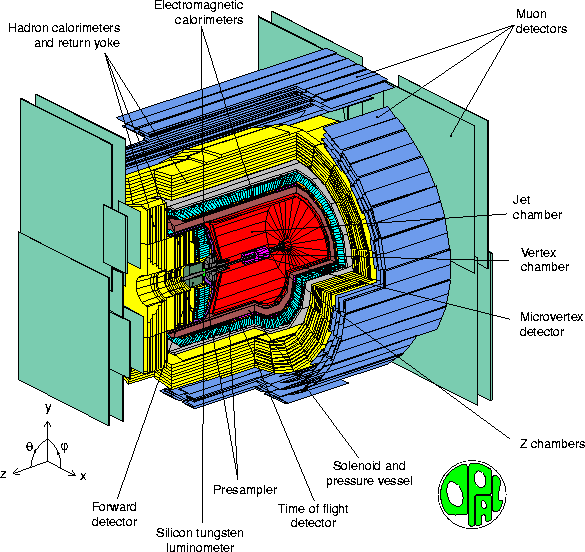
\includegraphics[width=1.0\linewidth]{figures/opal}
    \caption{The image shows a cut-away view of the \textbf{OPAL} detector\cite{CERN_OPAL}. The layered structure of the
    different chambers, which encase the central beam pipe, can be distinguished clearly. The beams are essentially
prepared to be mono-energetic. They collide at the center of the detector (near the Microvertex detector).}
    \label{fig:opal1}
\end{figure}

\begin{figure}[htpb]
    \centering
    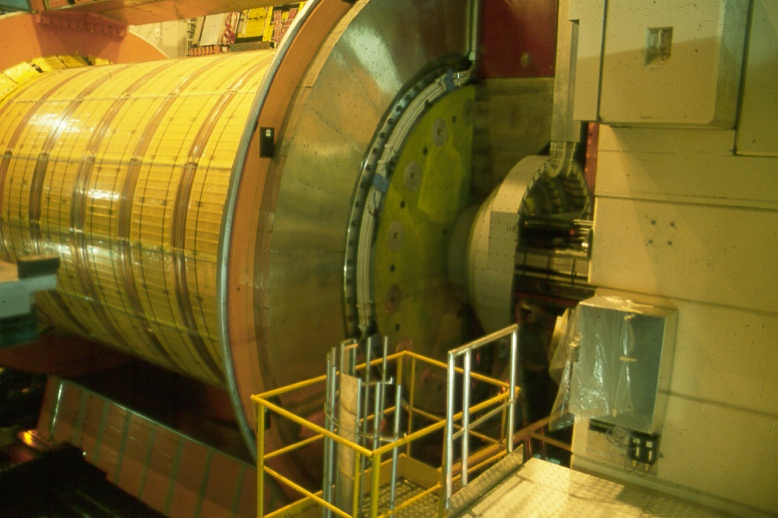
\includegraphics[width=1.0\linewidth]{figures/opal_photo}
    \caption{Photography of the early installation, spring 1988\cite{CERN_OPAL}. The experiments extents were
    $12m \times 12m \times 12m$ and was dismantled in 2001 due to to the construction of the LHC. To the right you can 
see outer structure of the detector, for more technical details refer to figure~\ref{fig:opal1}. }
    \label{fig:opal_photo}
\end{figure}

